\begin{figure}[H]
  \centering
  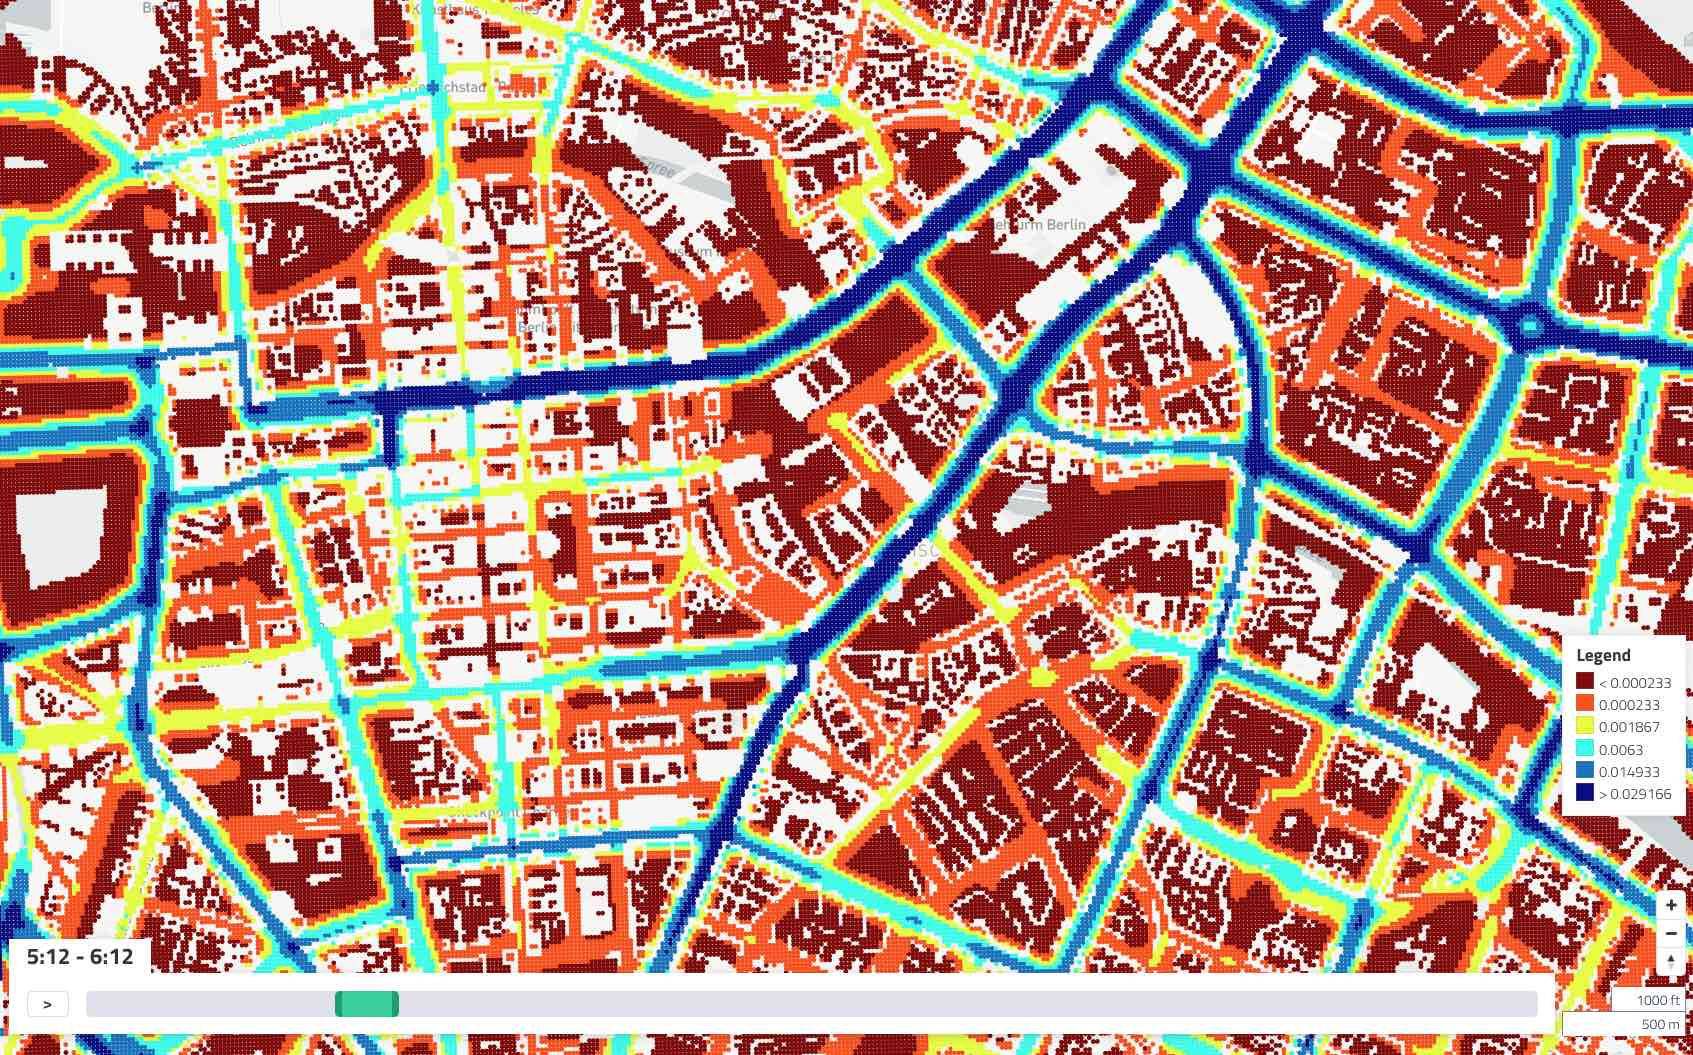
\includegraphics[width=0.8\textwidth]{assets/xyt-emissions.jpg}
  \caption{X/Y/Time point-based emissions data example}
\end{figure}

Display disaggregate point data with a time component; useful for
emissions, noise, etc.

We are currently researching the best way to ingest very large
X/Y/Time data files.

Currently, SimWrapper can load an \texttt{*.xyt.csv} file
but it takes a long time (up to a few minutes for some simulations), and
then the viz displays.

\hypertarget{usage}{%
\subsection{Usage}}

If a file with name matching \texttt{*.xyt.csv} exists in a folder, the
X/Y/T viewer will be available. There is no YAML configuration
available, but there is an interactive panel for modifying the color
attributes.
